% Created by tikzDevice version 0.12.6 on 2026-08-13 01:05:06
% !TEX encoding = UTF-8 Unicode
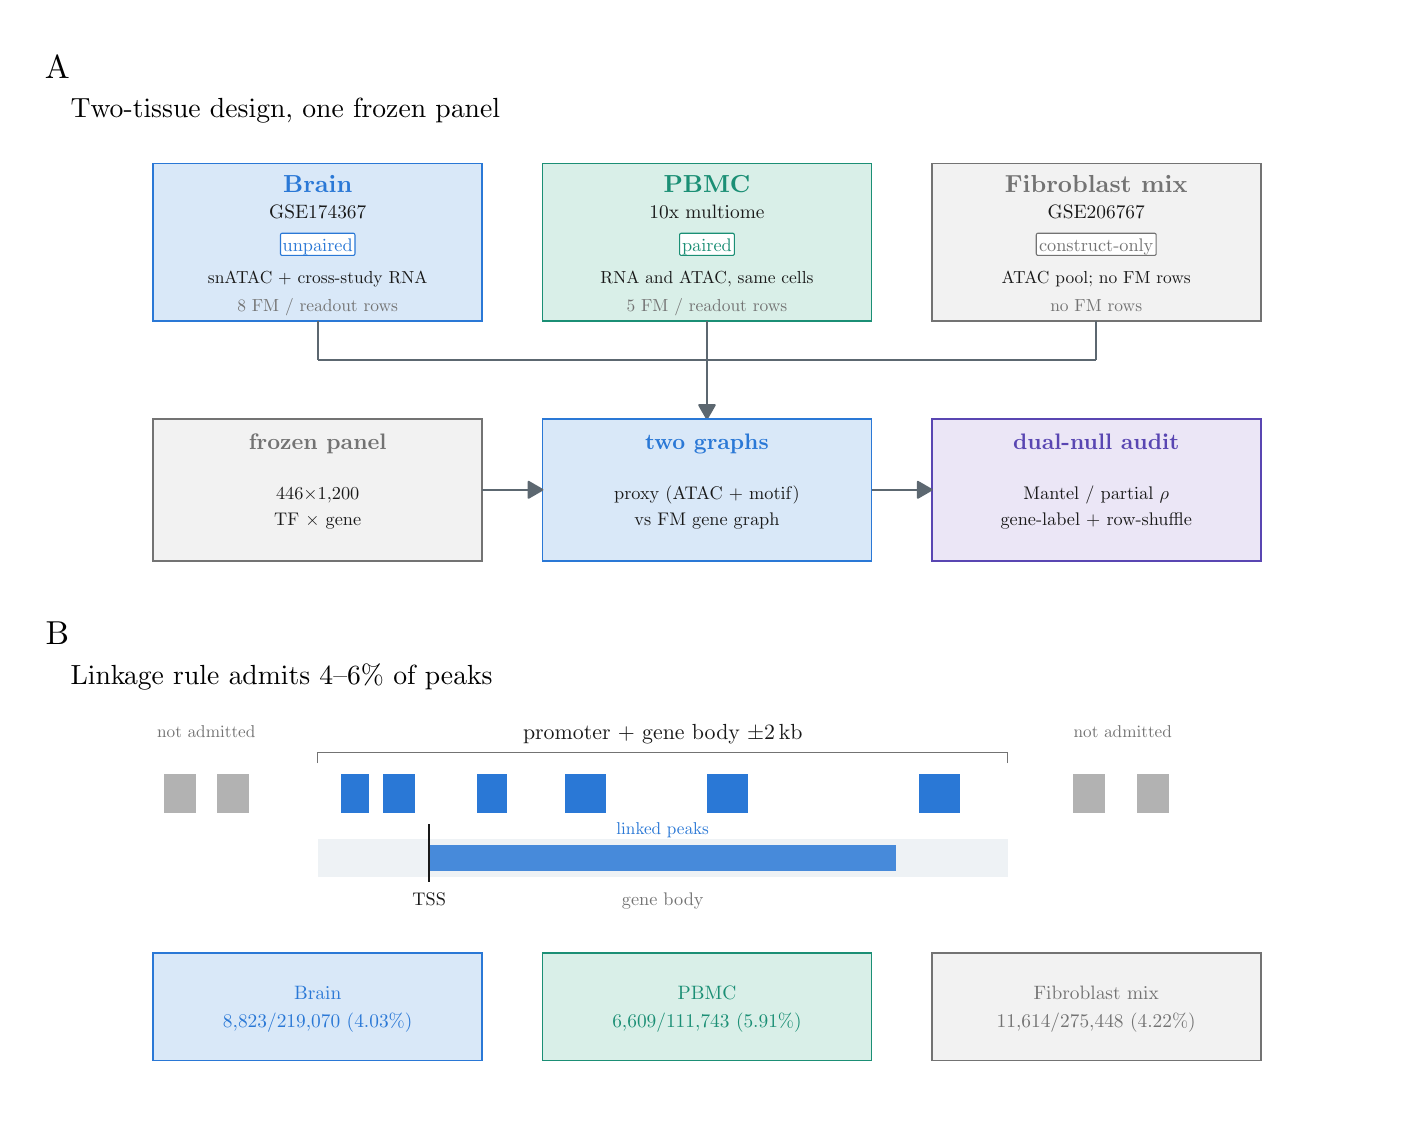
\begin{tikzpicture}[x=1pt,y=1pt]
\definecolor{fillColor}{RGB}{255,255,255}
\path[use as bounding box,fill=fillColor,fill opacity=0.00] (0,0) rectangle (491.44,390.26);
\begin{scope}
\path[clip] (  0.00,  0.00) rectangle (491.44,390.26);
\definecolor{drawColor}{RGB}{255,255,255}
\definecolor{fillColor}{RGB}{255,255,255}

\path[draw=drawColor,line width= 0.6pt,line join=round,line cap=round,fill=fillColor] (  0.00,  0.00) rectangle (491.44,390.26);
\end{scope}
\begin{scope}
\path[clip] (  4.00,181.53) rectangle (485.44,386.26);

\path[] (  4.00,181.53) rectangle (485.44,386.26);
\end{scope}
\begin{scope}
\path[clip] (  4.00,  3.00) rectangle (485.44,181.53);

\path[] (  4.00,  3.00) rectangle (485.44,181.53);
\end{scope}
\begin{scope}
\path[clip] (  0.00,  0.00) rectangle (491.44,390.26);
\definecolor{drawColor}{RGB}{42,120,214}
\definecolor{fillColor}{RGB}{217,232,248}

\path[draw=drawColor,line width= 0.6pt,fill=fillColor] ( 45.34,284.38) rectangle (164.26,341.14);
\definecolor{drawColor}{RGB}{27,143,117}
\definecolor{fillColor}{RGB}{217,239,232}

\path[draw=drawColor,line width= 0.6pt,fill=fillColor] (186.00,284.38) rectangle (304.92,341.14);
\definecolor{drawColor}{gray}{0.45}
\definecolor{fillColor}{gray}{0.95}

\path[draw=drawColor,line width= 0.6pt,fill=fillColor] (326.66,284.38) rectangle (445.58,341.14);
\definecolor{drawColor}{RGB}{42,120,214}

\node[text=drawColor,anchor=base,inner sep=0pt, outer sep=0pt, scale=  0.89] at (104.80,330.68) {\bfseries Brain};
\definecolor{drawColor}{RGB}{27,143,117}

\node[text=drawColor,anchor=base,inner sep=0pt, outer sep=0pt, scale=  0.89] at (245.46,330.68) {\bfseries PBMC};
\definecolor{drawColor}{gray}{0.45}

\node[text=drawColor,anchor=base,inner sep=0pt, outer sep=0pt, scale=  0.89] at (386.12,330.68) {\bfseries Fibroblast mix};
\definecolor{drawColor}{gray}{0.10}

\node[text=drawColor,anchor=base,inner sep=0pt, outer sep=0pt, scale=  0.70] at (104.80,321.21) {GSE174367};

\node[text=drawColor,anchor=base,inner sep=0pt, outer sep=0pt, scale=  0.70] at (245.46,321.21) {10x multiome};

\node[text=drawColor,anchor=base,inner sep=0pt, outer sep=0pt, scale=  0.70] at (386.12,321.21) {GSE206767};
\definecolor{drawColor}{RGB}{42,120,214}
\definecolor{fillColor}{RGB}{255,255,255}

\path[draw=drawColor,line width= 0.4pt,line join=round,line cap=round,fill=fillColor] ( 92.05,307.97) --
	(117.56,307.97) --
	(117.53,307.97) --
	(117.65,307.97) --
	(117.76,307.99) --
	(117.86,308.03) --
	(117.96,308.09) --
	(118.05,308.16) --
	(118.12,308.25) --
	(118.18,308.34) --
	(118.22,308.44) --
	(118.25,308.55) --
	(118.26,308.67) --
	(118.26,308.67) --
	(118.26,315.28) --
	(118.26,315.28) --
	(118.25,315.39) --
	(118.22,315.50) --
	(118.18,315.60) --
	(118.12,315.70) --
	(118.05,315.78) --
	(117.96,315.85) --
	(117.86,315.91) --
	(117.76,315.95) --
	(117.65,315.97) --
	(117.56,315.98) --
	( 92.05,315.98) --
	( 92.13,315.97) --
	( 92.02,315.98) --
	( 91.91,315.96) --
	( 91.80,315.93) --
	( 91.70,315.88) --
	( 91.61,315.82) --
	( 91.52,315.74) --
	( 91.46,315.65) --
	( 91.40,315.55) --
	( 91.37,315.44) --
	( 91.35,315.33) --
	( 91.35,315.28) --
	( 91.35,308.67) --
	( 91.35,308.72) --
	( 91.35,308.61) --
	( 91.37,308.50) --
	( 91.40,308.39) --
	( 91.46,308.29) --
	( 91.52,308.20) --
	( 91.61,308.12) --
	( 91.70,308.06) --
	( 91.80,308.01) --
	( 91.91,307.98) --
	( 92.02,307.97) --
	cycle;
\end{scope}
\begin{scope}
\path[clip] (  0.00,  0.00) rectangle (491.44,390.26);
\definecolor{drawColor}{RGB}{42,120,214}

\node[text=drawColor,anchor=base,inner sep=0pt, outer sep=0pt, scale=  0.66] at (104.80,309.53) {unpaired};
\end{scope}
\begin{scope}
\path[clip] (  0.00,  0.00) rectangle (491.44,390.26);
\definecolor{drawColor}{RGB}{27,143,117}
\definecolor{fillColor}{RGB}{255,255,255}

\path[draw=drawColor,line width= 0.4pt,line join=round,line cap=round,fill=fillColor] (236.26,307.97) --
	(254.66,307.97) --
	(254.63,307.97) --
	(254.75,307.97) --
	(254.86,307.99) --
	(254.96,308.03) --
	(255.06,308.09) --
	(255.15,308.16) --
	(255.22,308.25) --
	(255.28,308.34) --
	(255.32,308.44) --
	(255.35,308.55) --
	(255.36,308.67) --
	(255.36,308.67) --
	(255.36,315.28) --
	(255.36,315.28) --
	(255.35,315.39) --
	(255.32,315.50) --
	(255.28,315.60) --
	(255.22,315.70) --
	(255.15,315.78) --
	(255.06,315.85) --
	(254.96,315.91) --
	(254.86,315.95) --
	(254.75,315.97) --
	(254.66,315.98) --
	(236.26,315.98) --
	(236.35,315.97) --
	(236.23,315.98) --
	(236.12,315.96) --
	(236.01,315.93) --
	(235.91,315.88) --
	(235.82,315.82) --
	(235.74,315.74) --
	(235.67,315.65) --
	(235.62,315.55) --
	(235.58,315.44) --
	(235.57,315.33) --
	(235.56,315.28) --
	(235.56,308.67) --
	(235.57,308.72) --
	(235.57,308.61) --
	(235.58,308.50) --
	(235.62,308.39) --
	(235.67,308.29) --
	(235.74,308.20) --
	(235.82,308.12) --
	(235.91,308.06) --
	(236.01,308.01) --
	(236.12,307.98) --
	(236.23,307.97) --
	cycle;
\end{scope}
\begin{scope}
\path[clip] (  0.00,  0.00) rectangle (491.44,390.26);
\definecolor{drawColor}{RGB}{27,143,117}

\node[text=drawColor,anchor=base,inner sep=0pt, outer sep=0pt, scale=  0.66] at (245.46,309.53) {paired};
\end{scope}
\begin{scope}
\path[clip] (  0.00,  0.00) rectangle (491.44,390.26);
\definecolor{drawColor}{gray}{0.45}
\definecolor{fillColor}{RGB}{255,255,255}

\path[draw=drawColor,line width= 0.4pt,line join=round,line cap=round,fill=fillColor] (365.15,307.97) --
	(407.08,307.97) --
	(407.06,307.97) --
	(407.17,307.97) --
	(407.28,307.99) --
	(407.38,308.03) --
	(407.48,308.09) --
	(407.57,308.16) --
	(407.64,308.25) --
	(407.70,308.34) --
	(407.75,308.44) --
	(407.77,308.55) --
	(407.78,308.67) --
	(407.78,308.67) --
	(407.78,315.28) --
	(407.78,315.28) --
	(407.77,315.39) --
	(407.75,315.50) --
	(407.70,315.60) --
	(407.64,315.70) --
	(407.57,315.78) --
	(407.48,315.85) --
	(407.38,315.91) --
	(407.28,315.95) --
	(407.17,315.97) --
	(407.08,315.98) --
	(365.15,315.98) --
	(365.24,315.97) --
	(365.13,315.98) --
	(365.01,315.96) --
	(364.91,315.93) --
	(364.80,315.88) --
	(364.71,315.82) --
	(364.63,315.74) --
	(364.56,315.65) --
	(364.51,315.55) --
	(364.47,315.44) --
	(364.46,315.33) --
	(364.45,315.28) --
	(364.45,308.67) --
	(364.46,308.72) --
	(364.46,308.61) --
	(364.47,308.50) --
	(364.51,308.39) --
	(364.56,308.29) --
	(364.63,308.20) --
	(364.71,308.12) --
	(364.80,308.06) --
	(364.91,308.01) --
	(365.01,307.98) --
	(365.13,307.97) --
	cycle;
\end{scope}
\begin{scope}
\path[clip] (  0.00,  0.00) rectangle (491.44,390.26);
\definecolor{drawColor}{gray}{0.45}

\node[text=drawColor,anchor=base,inner sep=0pt, outer sep=0pt, scale=  0.66] at (386.12,309.53) {construct-only};
\end{scope}
\begin{scope}
\path[clip] (  0.00,  0.00) rectangle (491.44,390.26);
\definecolor{drawColor}{gray}{0.10}

\node[text=drawColor,anchor=base,inner sep=0pt, outer sep=0pt, scale=  0.63] at (104.80,297.80) {snATAC + cross-study RNA};

\node[text=drawColor,anchor=base,inner sep=0pt, outer sep=0pt, scale=  0.63] at (245.46,297.80) {RNA and ATAC, same cells};

\node[text=drawColor,anchor=base,inner sep=0pt, outer sep=0pt, scale=  0.63] at (386.12,297.80) {ATAC pool; no FM rows};
\definecolor{drawColor}{gray}{0.45}

\node[text=drawColor,anchor=base,inner sep=0pt, outer sep=0pt, scale=  0.63] at (104.80,287.55) {8 FM / readout rows};

\node[text=drawColor,anchor=base,inner sep=0pt, outer sep=0pt, scale=  0.63] at (245.46,287.55) {5 FM / readout rows};

\node[text=drawColor,anchor=base,inner sep=0pt, outer sep=0pt, scale=  0.63] at (386.12,287.55) {no FM rows};
\definecolor{drawColor}{RGB}{92,103,112}

\path[draw=drawColor,line width= 0.6pt,line join=round] (104.80,284.38) -- (104.80,270.18);

\path[draw=drawColor,line width= 0.6pt,line join=round] (245.46,284.38) -- (245.46,270.18);

\path[draw=drawColor,line width= 0.6pt,line join=round] (386.12,284.38) -- (386.12,270.18);

\path[draw=drawColor,line width= 0.6pt,line join=round] (104.80,270.18) -- (386.12,270.18);

\path[draw=drawColor,line width= 0.6pt,line join=round] (245.46,270.18) -- (245.46,248.89);
\definecolor{fillColor}{RGB}{92,103,112}

\path[draw=drawColor,line width= 0.6pt,line join=round,fill=fillColor] (242.57,253.90) --
	(245.46,248.89) --
	(248.35,253.90) --
	cycle;
\definecolor{drawColor}{gray}{0.45}
\definecolor{fillColor}{gray}{0.95}

\path[draw=drawColor,line width= 0.6pt,fill=fillColor] ( 45.34,197.64) rectangle (164.26,248.89);
\definecolor{drawColor}{RGB}{42,120,214}
\definecolor{fillColor}{RGB}{217,232,248}

\path[draw=drawColor,line width= 0.6pt,fill=fillColor] (186.00,197.64) rectangle (304.92,248.89);
\definecolor{drawColor}{RGB}{89,70,178}
\definecolor{fillColor}{RGB}{235,230,246}

\path[draw=drawColor,line width= 0.6pt,fill=fillColor] (326.66,197.64) rectangle (445.58,248.89);
\definecolor{drawColor}{gray}{0.45}

\node[text=drawColor,anchor=base,inner sep=0pt, outer sep=0pt, scale=  0.81] at (104.80,237.94) {\bfseries frozen panel};
\definecolor{drawColor}{RGB}{42,120,214}

\node[text=drawColor,anchor=base,inner sep=0pt, outer sep=0pt, scale=  0.81] at (245.46,237.94) {\bfseries two graphs};
\definecolor{drawColor}{RGB}{89,70,178}

\node[text=drawColor,anchor=base,inner sep=0pt, outer sep=0pt, scale=  0.81] at (386.12,237.94) {\bfseries dual-null audit};
\definecolor{drawColor}{gray}{0.10}

\node[text=drawColor,anchor=base,inner sep=0pt, outer sep=0pt, scale=  0.66] at (104.80,219.62) {446$\times$1{,}200};

\node[text=drawColor,anchor=base,inner sep=0pt, outer sep=0pt, scale=  0.66] at (104.80,210.21) {TF $\times$ gene};

\node[text=drawColor,anchor=base,inner sep=0pt, outer sep=0pt, scale=  0.66] at (245.46,219.62) {proxy (ATAC + motif)};

\node[text=drawColor,anchor=base,inner sep=0pt, outer sep=0pt, scale=  0.66] at (245.46,210.21) {vs FM gene graph};

\node[text=drawColor,anchor=base,inner sep=0pt, outer sep=0pt, scale=  0.66] at (386.12,219.62) {Mantel / partial $\rho$};

\node[text=drawColor,anchor=base,inner sep=0pt, outer sep=0pt, scale=  0.66] at (386.12,210.21) {gene-label + row-shuffle};
\definecolor{drawColor}{RGB}{92,103,112}

\path[draw=drawColor,line width= 0.7pt,line join=round] (164.26,223.27) -- (186.00,223.27);
\definecolor{fillColor}{RGB}{92,103,112}

\path[draw=drawColor,line width= 0.7pt,line join=round,fill=fillColor] (180.99,220.38) --
	(186.00,223.27) --
	(180.99,226.16) --
	cycle;

\path[draw=drawColor,line width= 0.7pt,line join=round] (304.92,223.27) -- (326.66,223.27);

\path[draw=drawColor,line width= 0.7pt,line join=round,fill=fillColor] (321.65,220.38) --
	(326.66,223.27) --
	(321.65,226.16) --
	cycle;
\end{scope}
\begin{scope}
\path[clip] (  0.00,  0.00) rectangle (491.44,390.26);
\definecolor{drawColor}{RGB}{0,0,0}

\node[text=drawColor,anchor=base west,inner sep=0pt, outer sep=0pt, scale=  1.00] at ( 15.49,357.63) {Two-tissue design, one frozen panel};
\end{scope}
\begin{scope}
\path[clip] (  0.00,  0.00) rectangle (491.44,390.26);
\definecolor{drawColor}{RGB}{0,0,0}

\node[text=drawColor,anchor=base,inner sep=0pt, outer sep=0pt, scale=  1.20] at ( 10.74,371.95) {A};
\end{scope}
\begin{scope}
\path[clip] (  0.00,  0.00) rectangle (491.44,390.26);
\definecolor{fillColor}{RGB}{238,242,245}

\path[fill=fillColor] (104.80, 83.21) rectangle (354.15, 97.22);
\definecolor{fillColor}{RGB}{42,120,214}

\path[fill=fillColor,fill opacity=0.85] (145.08, 85.55) rectangle (313.87, 94.89);
\definecolor{drawColor}{gray}{0.10}

\path[draw=drawColor,line width= 0.6pt,line join=round] (145.08, 81.66) -- (145.08,102.67);
\definecolor{fillColor}{gray}{0.70}

\path[fill=fillColor] ( 49.18,106.56) rectangle ( 60.69,120.57);

\path[fill=fillColor] ( 68.36,106.56) rectangle ( 79.87,120.57);
\definecolor{fillColor}{RGB}{42,120,214}

\path[fill=fillColor] (113.12,106.56) rectangle (123.35,120.57);

\path[fill=fillColor] (128.46,106.56) rectangle (139.97,120.57);

\path[fill=fillColor] (162.35,106.56) rectangle (173.21,120.57);

\path[fill=fillColor] (194.31,106.56) rectangle (209.02,120.57);

\path[fill=fillColor] (245.46,106.56) rectangle (260.17,120.57);

\path[fill=fillColor] (322.18,106.56) rectangle (336.89,120.57);
\definecolor{fillColor}{gray}{0.70}

\path[fill=fillColor] (377.81,106.56) rectangle (389.32,120.57);

\path[fill=fillColor] (400.82,106.56) rectangle (412.33,120.57);
\definecolor{drawColor}{gray}{0.45}

\path[draw=drawColor,line width= 0.5pt,line join=round] (104.80,128.35) -- (354.15,128.35);

\path[draw=drawColor,line width= 0.5pt,line join=round] (104.80,124.46) -- (104.80,128.35);

\path[draw=drawColor,line width= 0.5pt,line join=round] (354.15,124.46) -- (354.15,128.35);
\definecolor{drawColor}{gray}{0.10}

\node[text=drawColor,anchor=base,inner sep=0pt, outer sep=0pt, scale=  0.79] at (229.48,133.21) {promoter + gene body $\pm$2\,kb};

\node[text=drawColor,anchor=base,inner sep=0pt, outer sep=0pt, scale=  0.66] at (145.08, 72.99) {TSS};
\definecolor{drawColor}{gray}{0.45}

\node[text=drawColor,anchor=base,inner sep=0pt, outer sep=0pt, scale=  0.66] at (229.48, 72.99) {gene body};

\node[text=drawColor,anchor=base,inner sep=0pt, outer sep=0pt, scale=  0.62] at ( 64.53,133.84) {not admitted};

\node[text=drawColor,anchor=base,inner sep=0pt, outer sep=0pt, scale=  0.62] at (395.71,133.84) {not admitted};
\definecolor{drawColor}{RGB}{42,120,214}

\node[text=drawColor,anchor=base,inner sep=0pt, outer sep=0pt, scale=  0.62] at (229.48, 98.82) {linked peaks};
\definecolor{fillColor}{RGB}{217,232,248}

\path[draw=drawColor,line width= 0.6pt,fill=fillColor] ( 45.34, 17.06) rectangle (164.26, 55.97);
\definecolor{drawColor}{RGB}{27,143,117}
\definecolor{fillColor}{RGB}{217,239,232}

\path[draw=drawColor,line width= 0.6pt,fill=fillColor] (186.00, 17.06) rectangle (304.92, 55.97);
\definecolor{drawColor}{gray}{0.45}
\definecolor{fillColor}{gray}{0.95}

\path[draw=drawColor,line width= 0.6pt,fill=fillColor] (326.66, 17.06) rectangle (445.58, 55.97);
\definecolor{drawColor}{RGB}{42,120,214}

\node[text=drawColor,anchor=base,inner sep=0pt, outer sep=0pt, scale=  0.70] at (104.80, 39.00) {Brain};

\node[text=drawColor,anchor=base,inner sep=0pt, outer sep=0pt, scale=  0.70] at (104.80, 28.86) {8,823/219,070 (4.03\%)};
\definecolor{drawColor}{RGB}{27,143,117}

\node[text=drawColor,anchor=base,inner sep=0pt, outer sep=0pt, scale=  0.70] at (245.46, 39.00) {PBMC};

\node[text=drawColor,anchor=base,inner sep=0pt, outer sep=0pt, scale=  0.70] at (245.46, 28.86) {6,609/111,743 (5.91\%)};
\definecolor{drawColor}{gray}{0.45}

\node[text=drawColor,anchor=base,inner sep=0pt, outer sep=0pt, scale=  0.70] at (386.12, 39.00) {Fibroblast mix};

\node[text=drawColor,anchor=base,inner sep=0pt, outer sep=0pt, scale=  0.70] at (386.12, 28.86) {11,614/275,448 (4.22\%)};
\end{scope}
\begin{scope}
\path[clip] (  0.00,  0.00) rectangle (491.44,390.26);
\definecolor{drawColor}{RGB}{0,0,0}

\node[text=drawColor,anchor=base west,inner sep=0pt, outer sep=0pt, scale=  1.00] at ( 15.49,152.90) {Linkage rule admits 4--6\% of peaks};
\end{scope}
\begin{scope}
\path[clip] (  0.00,  0.00) rectangle (491.44,390.26);
\definecolor{drawColor}{RGB}{0,0,0}

\node[text=drawColor,anchor=base,inner sep=0pt, outer sep=0pt, scale=  1.20] at ( 10.74,167.23) {B};
\end{scope}
\end{tikzpicture}
